\begin{trapbox}
\par\noindent\begin{minipage}{\linewidth}
\textbf{容易犯的错误不是“公式太难”，而是没有分清边、点和方向。}
\begin{enumerate}
\item \textbf{系数与顶点配错。}误写 $b\vec{IA}+c\vec{IB}+a\vec{IC}=\vec0$。\textbf{正确：}$A$ 对应 $BC=a$，$B$ 对应 $CA=b$，$C$ 对应 $AB=c$。核对方法：系数来自\textbf{不包含该顶点}的小三角形底边。
% a=10,b=8,c=6. Wrong cyclic weights give J=(bA+cB+aC)/24=(3/2,10/3).
\begin{center}
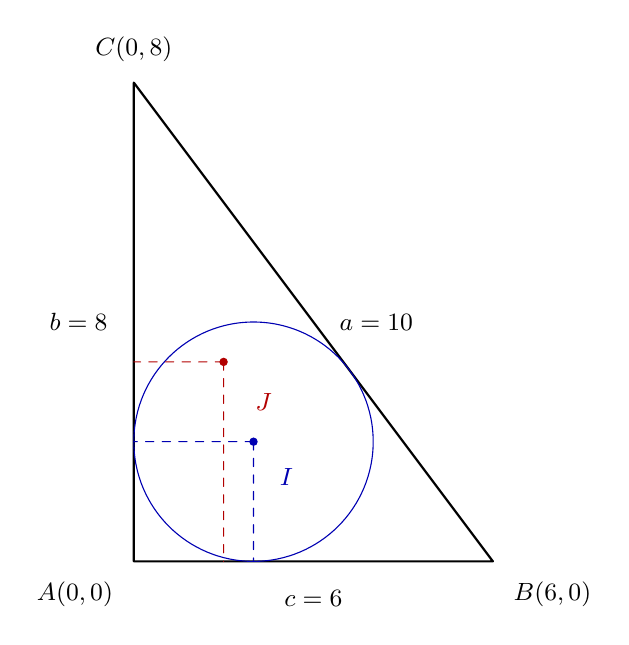
\begin{tikzpicture}[scale=.76,font=\small,line cap=round,line join=round]
\coordinate (A) at (0,0);\coordinate (B) at (6,0);\coordinate (C) at (0,8);
\coordinate (I) at (2,2);\coordinate (J) at (1.5,10/3);
\draw[thick] (A)--(B)--(C)--cycle;
\draw[blue!70!black] (I) circle[radius=2];
\draw[blue!70!black,dashed] (I)--(2,0) (I)--(0,2);
\draw[red!70!black,dashed] (J)--(1.5,0) (J)--(0,10/3);
\fill[blue!70!black] (I) circle[radius=2pt];\node[below right=6pt,blue!70!black] at (I) {$I$};
\fill[red!70!black] (J) circle[radius=2pt];\node[below right=8pt,red!70!black] at (J) {$J$};
\node[below left=4pt] at (A) {$A(0,0)$};\node[below right=4pt] at (B) {$B(6,0)$};\node[above=4pt] at (C) {$C(0,8)$};
\path (B)--node[midway,right=6pt] {$a=10$} (C);
\path (C)--node[midway,left=6pt] {$b=8$} (A);
\path (A)--node[midway,below=7pt] {$c=6$} (B);
\end{tikzpicture}
\par\smallskip{\small 正确内心 $I(2,2)$；错配系数得到 $J(3/2,10/3)$，它到两坐标轴的距离都不相等。}
\end{center}

图中若把系数错排为 $b,c,a$，坐标式就给出 $J=(bA+cB+aC)/(a+b+c)$；它不是内心。
\end{enumerate}
\end{minipage}\par
\begin{enumerate}[start=2]
\item \textbf{把内心当重心。} $\vec{OI}=(\vec{OA}+\vec{OB}+\vec{OC})/3$ 通常是重心公式，不是内心公式。只有特殊情况才重合。
\item \begin{minipage}[t]{\linewidth}\textbf{把角平分线方向当作内心坐标。} $\vec{AB}/c+\vec{AC}/b$ 仅确定\textbf{从 $A$ 出发的角平分线方向}，不直接说明 $I=A+\vec{AB}/c+\vec{AC}/b$。还必须知道在该方向走多远。
% Same axes and true lengths: A=(0,0),B=(6,0),C=(0,8),I=(2,2).
\begin{center}
\begin{tikzpicture}[scale=.78,font=\small,>=Stealth,line cap=round,line join=round]
\coordinate (A) at (0,0);\coordinate (B) at (6,0);\coordinate (C) at (0,8);
\coordinate (I) at (2,2);\coordinate (Q) at (1,1);
\draw[->,gray!75] (-.7,0)--(7,0) node[right] {$x$};
\draw[->,gray!75] (0,-.7)--(0,8.8) node[above] {$y$};
\draw[thick] (A)--(B)--(C)--cycle;
\draw[blue!70!black] (I) circle[radius=2];
\draw[->,green!45!black,thick] (A)--(4.2,4.2) node[right=5pt] {同一方向};
\draw[->,blue!70!black,very thick] (A)--(1,0);
\draw[->,orange!80!black,very thick] (A)--(0,1);
\fill[red!70!black] (Q) circle[radius=2pt];\node[right=10pt,red!70!black] at (Q) {$Q$};
\fill[blue!70!black] (I) circle[radius=2pt];\node[above left=6pt,blue!70!black] at (I) {$I$};
\node[below left=4pt] at (A) {$A(0,0)$};\node[below=5pt] at (B) {$B(6,0)$};
\node[above left=4pt] at (C) {$C(0,8)$};
\end{tikzpicture}
\par\smallskip{\small $\vec u=(1,0),\ \vec v=(0,1)$；$A+\vec u+\vec v=Q(1,1)$，内心却是 $I(2,2)$，不能把方向当位置。}
\end{center}

\end{minipage}
\item \textbf{忘记向量起点。}自由向量本身不能说“经过内心”。准确说法是\textbf{过顶点 $A$、与该向量平行的直线}经过内心。
\item \textbf{角平分线分点系数写反。}若 $BD:DC=c:b$，则
\[\vec{BD}=\frac c{b+c}\vec{BC},\quad
\vec{AD}=\frac b{b+c}\vec{AB}+\frac c{b+c}\vec{AC}.\]
$\vec{AD}$ 中 $\vec{AB}$ 前的系数是 $b$，不是 $c$：由 $\vec{AD}=\vec{AB}+\vec{BD}$ 重新推一次即可校验。
\item \textbf{把向量大小比直接当作向量等式。} $AI:ID=(b+c):a$ 只是长度比；因为 $\vec{IA},\vec{ID}$ 反向，必须有\[\vec{IA}=-\frac{b+c}{a}\vec{ID}.\]
\item \textbf{反向判断时没有检验系数。} $2\vec{PA}+3\vec{PB}+4\vec{PC}=0$ 不会对所有三角形都说明 $P$ 是内心。需要先计算 $a:b:c$，确认比例一致；若出现负系数，也不能直接使用内心结论。
\item \begin{minipage}[t]{\linewidth}\textbf{把“内心在三角形内”漏掉。}单靠“到三条边所在直线的距离相等”，还可能出现\textbf{三角形外部的等距点}。如果用距离相等的办法验证，必须同时证明点在三角形内部。
% A=(0,0), B=(4,0), C=(0,3); I=(1,1), exterior equidistant point J=(-2,2).
\begin{center}
\begin{tikzpicture}[scale=.9,font=\small,line cap=round,line join=round]
\coordinate (A) at (0,0);\coordinate (B) at (4,0);\coordinate (C) at (0,3);
\coordinate (I) at (1,1);\coordinate (J) at (-2,2);
\coordinate (X) at (-2,0);\coordinate (Y) at (0,2);
\coordinate (F) at ($(C)!(J)!(B)$);
\fill[blue!6] (A)--(B)--(C)--cycle;\draw[thick] (A)--(B)--(C)--cycle;
\draw[dashed,gray!75] (-4.5,0)--(A) (C)--(-1.8,4.35);
\draw[blue!70!black,thick] (I) circle[radius=1];
\draw[orange!85!black,thick] (J) circle[radius=2];
\draw[orange!85!black,thick] (J)--node[midway,left=5pt] {$2$} (X);
\draw[orange!85!black,thick] (J)--node[midway,below=5pt] {$2$} (Y);
\draw[orange!85!black,thick] (J)--node[pos=.6,above left=4pt] {$2$} (F);
\pic[draw,angle radius=2.5mm] {right angle=J--F--B};
\pic[draw,angle radius=2.5mm] {right angle=J--X--B};
\pic[draw,angle radius=2.5mm] {right angle=J--Y--A};
\fill (I) circle[radius=2pt];\node[above right=5pt,blue!70!black] at (I) {$I$};
\fill (J) circle[radius=2pt];\node[above left=5pt,orange!85!black] at (J) {$J$};
\node[below left=4pt] at (A) {$A$};\node[right=5pt] at (B) {$B(4,0)$};\node[above right=7pt] at (C) {$C(0,3)$};
\end{tikzpicture}
\par\smallskip{\small 内心 $I(1,1)$ 在内部；$J(-2,2)$ 到三条边所在直线均距 $2$，到 $AB,BC$ 的垂足在延长线上。}
\end{center}

\end{minipage}
\item \textbf{内外角平分线搞混。} $\vec u+\vec v$ 与 $\vec u-\vec v$（$\vec u,\vec v$ 为长度为 $1$ 的两边方向向量）分别表示内、外角平分线方向；减法得到的直线通常\textbf{不经过内心}。
\item \textbf{没有检查三角形是否真的存在。} 边长需要满足任意两边之和大于第三边；三点不能共线。否则\textbf{内心与内切圆}的讨论没有通常意义。
\end{enumerate}
\end{trapbox}
